\documentclass[a4paper]{article}
\usepackage{vntex}
%\usepackage[enetglish,vinam]{babel}
%\usepackage[utf8]{inputenc}
\usepackage{mathptmx}[ptm]
%\usepackage[utf8]{inputenc}
%\usepackage[francais]{babel}
\usepackage{a4wide,amssymb,epsfig,latexsym,array,hhline,fancyhdr}
\usepackage[normalem]{ulem}
%\usepackage{soul}

\usepackage[makeroom]{cancel}
\usepackage{amsmath}
\usepackage{amsthm}
\usepackage{multicol,longtable,amscd}
\usepackage{diagbox}%Make diagonal lines in tables
\usepackage{booktabs}
\usepackage{alltt}
\usepackage[framemethod=tikz]{mdframed}% For highlighting paragraph backgrounds
\usepackage{caption,subcaption}

\usepackage{lastpage}
\usepackage[lined,boxed,commentsnumbered]{algorithm2e}
\usepackage{enumerate}
\usepackage{color}
\usepackage{graphicx}							% Standard graphics package
\usepackage{array}
\usepackage{tabularx, caption}
\usepackage{multirow}
\usepackage{multicol}
\usepackage{rotating}
\usepackage{graphics}
\usepackage{geometry}
\usepackage{setspace}
\usepackage{epsfig}
\usepackage{tikz}

\usetikzlibrary{arrows,snakes,backgrounds,calc}
\usepackage[unicode]{hyperref}
\hypersetup{urlcolor=blue,linkcolor=black,citecolor=black,colorlinks=true} 
\usepackage{listings}

%\usepackage{pstcol} 								% PSTricks with the standard color package

\usepackage[normalem]{ulem}

\newtheorem{theorem}{{\bf Định lý}}
\newtheorem{property}{{\bf Tính chất}}
\newtheorem{proposition}{{\bf Mệnh đề}}
\newtheorem{corollary}[proposition]{{\bf Hệ quả}}
\newtheorem{lemma}[proposition]{{\bf Bổ đề}}
\theoremstyle{definition}
\newtheorem{exer}{Bài toán}
\addtocontents{toc}{\protect\thispagestyle{empty}}
% Remove page number in contents page. 
\addtocontents{lof}{\protect\thispagestyle{empty}}
% Remove page number in list of figure page. 
\addtocontents{lot}{\protect\thispagestyle{empty}}
% Remove page number in list of table page. 
\def\thesislayout{	% A4: 210 × 297
	\geometry{
		a4paper,
		total={160mm,240mm},  % fix over page
		left=30mm,
		top=22mm,
            right=20mm,
            bottom=20mm,
	}
}
\def\thesisheadlayout{	% A4: 210 × 297
	\geometry{
		a4paper,
		total={160mm,240mm},  % fix over page
		left=30mm,
		top=10mm,
	}
}
\thesislayout
\lstset{
language=R,
basicstyle=\footnotesize\sffamily,
commentstyle=\ttfamily\color{black},
numbers=left,
numberstyle=\ttfamily\color{black}\footnotesize,
stepnumber=1,
numbersep=5pt,
backgroundcolor=\color{white},
showspaces=false,
showstringspaces=false,
showtabs=false,
frame=single,
tabsize=2,
captionpos=b,
breaklines=true,
breakatwhitespace=false,
title=\lstname,
escapeinside={},
keywordstyle={},
morekeywords={}
}
%\usepackage{fancyhdr}
\setlength{\headheight}{40pt}
\pagestyle{fancy}
\fancyhead{} % clear all header fields
\renewcommand{\footruleskip}{1mm}

\fancyhead[L]{
 \begin{tabular}{rl}
    \begin{picture}(25,15)(0,0)
    \put(0,-8){
\includegraphics[width=10mm, height=10mm]{Images/hcmut.png}}
    %\put(0,-8){\epsfig{width=10mm,figure=hcmut.eps}}
   \end{picture}&
	%
\includegraphics[width=8mm, height=8mm]{hcmut.png} & %
	\begin{tabular}{l}
		\textbf{  Trường Đại Học Bách Khoa - Đại học Quốc gia TP.HCM }\\
		\textbf{  Khoa Khoa Học \& Kỹ Thuật Máy Tính}
	\end{tabular} 	
 \end{tabular}
}
\fancyhead[R]{
	\begin{tabular}{l}
		\tiny \bf \\
		\tiny \bf 
	\end{tabular}  }
\fancyfoot{} % clear all footer fields
\fancyfoot[L]{\scriptsize  Báo cáo Bài tập lớn Khai phá dữ liệu - HK2 2024 - 2025}
\fancyfoot[R]{\scriptsize  Trang {\thepage}/\pageref{LastPage}}

\renewcommand{\headrulewidth}{0.3pt}
\renewcommand{\footrulewidth}{0.3pt}

%%%
\setcounter{secnumdepth}{4}
\setcounter{tocdepth}{3}
\makeatletter
\newcounter {subsubsubsection}[subsubsection]
\renewcommand\thesubsubsubsection{\thesubsubsection .\@alph\c@subsubsubsection}
\newcommand\subsubsubsection{\@startsection{subsubsubsection}{4}{\z@}%
                                     {-3.25ex\@plus -1ex \@minus -.2ex}%
                                     {1.5ex \@plus .2ex}%
                                     {\normalfont\normalsize\bfseries}}
\newcommand*\l@subsubsubsection{\@dottedtocline{3}{10.0em}{4.1em}}
\newcommand*{\subsubsubsectionmark}[1]{}
\makeatother

\everymath{\color{black}}%make in-line maths symbols blue to read/check easily

\sloppy
\captionsetup[figure]{labelfont={small,bf},textfont={small,it},belowskip=-1pt,aboveskip=-9pt}
%space remove between caption, figure, and text
\captionsetup[table]{labelfont={small,bf},textfont={small,it},belowskip=-1pt,aboveskip=7pt}
\setlength{\floatsep}{5pt plus 2pt minus 2pt}
\setlength{\textfloatsep}{5pt plus 2pt minus 2pt}
\setlength{\intextsep}{10pt plus 2pt minus 2pt}

\thesislayout
\onehalfspacing

\begin{document}

\begin{titlepage}
\begin{tikzpicture}[remember picture, overlay]
  \draw[line width = 4pt] ($(current page.north west) + (0.4in,-0.5in)$) rectangle ($(current page.south east) + (-0.4in,0.5in)$);
  \draw[line width=1.5pt]
    ($ (current page.north west) + (0.45in,-0.55in) $)
    rectangle
    ($ (current page.south east) + (-0.45in,0.55in) $);
\end{tikzpicture}

\begin{center}
\LARGE \textbf{ĐẠI HỌC QUỐC GIA THÀNH PHỐ HỒ CHÍ MINH} \\
\vspace{0.2cm}
\LARGE \textbf{TRƯỜNG ĐẠI HỌC BÁCH KHOA} \\
\vspace{0.2cm}
\LARGE \textbf{KHOA KHOA HỌC VÀ KĨ THUẬT MÁY TÍNH}
\end{center}

\vspace{0.3cm}

\begin{figure}[h!]
\begin{center}

\includegraphics[width=4cm]{Images/hcmut.png}
\end{center}
\end{figure}

\begin{center}
\begin{tabular}{c}
\textbf{{\LARGE BÁO CÁO BÀI TẬP LỚN}} \\
\\
\textbf{{\LARGE KHAI PHÁ DỮ LIỆU}} \\[15pt]
\\
\parbox{0.9\textwidth}{%
    \centering
    \textbf{\LARGE PHÂN TÍCH CÁC YẾU TỐ ẢNH HƯỞNG TỚI GIÁ \\[6pt] NÔNG SẢN VÀ XÂY DỰNG MÔ HÌNH DỰ ĐOÁN}
}
\end{tabular}
\end{center}

\vspace{0.5cm}
\begin{table}[h]
\begin{tabular}{rll}
\\
\\
\hspace{3 cm} &   \textbf{\Large GVHD:} {\Large Bùi Tiến Đức}
\\
\\
\\
\hspace{3 cm} &     \textbf{$\;$ $\;$$\;$$\;$$\;$$\;$$\;$$\;$$\;$$\;$$\;$$\;$$\;$$\;$$\;$$\;$$\;$$\;$$\;$$\;$$\;$$\;$$\;$$\;$$\;$$\;$$\;$$\;$$\;$$\;$$\;$$\;$$\;$$\;$ \Large ---o0o---} 
\\
\\
\hspace{3 cm} &   \textbf{\Large SVTH1:  } {\Large Phan Nguyễn Hữu Phước - 2212720}
\\
\\
\hspace{3 cm}&   \textbf{\Large SVTH2:  }  {\Large .....Họ \& Tên...........(MSSV)}
\\
\\
\end{tabular}
\end{table}
\vspace{0.5cm}
\begin{center}
{\Large TP. HỒ CHÍ MINH, THÁNG 4/2025 }
\end{center}
\end{titlepage}
%\thispagestyle{empty}
\newpage
%%%%%%%%%%%%%%%%%INTRO%%%%%%%%%%%%%%%%%%%
\newpage
\tableofcontents
\newpage
\listoffigures
\newpage
\listoftables
\newpage
\setcounter{page}{1}

%%%%%%%%%%%%%%%%%CONTENTS%%%%%%%%%%%%%%%%%%%
\input{Contents/1.GioiThieu}
\newpage
\section{Tổng quan công việc}

\subsection{Giới thiệu về phương pháp luận}

\hspace{0.5cm}Trong dự án này, chúng tôi áp dụng phương pháp luận CRISP-DM (Cross-Industry Standard Process for Data Mining) để thực hiện quá trình khai thác dữ liệu. Phương pháp này bao gồm 6 giai đoạn chính:

\begin{itemize}
    \item \textbf{Hiểu biết về nghiệp vụ (Business Understanding):} Xác định mục tiêu và yêu cầu của dự án
    \item \textbf{Hiểu biết về dữ liệu (Data Understanding):} Thu thập và phân tích dữ liệu ban đầu
    \item \textbf{Chuẩn bị dữ liệu (Data Preparation):} Tiền xử lý và làm sạch dữ liệu
    \item \textbf{Mô hình hóa (Modeling):} Xây dựng và đánh giá các mô hình
    \item \textbf{Đánh giá (Evaluation):} Đánh giá kết quả và kiểm tra mục tiêu
    \item \textbf{Triển khai (Deployment):} Triển khai và duy trì mô hình
\end{itemize}

\subsection{Phương pháp tiếp cận}

\hspace{0.5cm}Dự án sử dụng phương pháp tiếp cận dựa trên dữ liệu (Data-Driven Approach) để phân tích và dự đoán năng suất cây trồng. Các bước thực hiện bao gồm:

\begin{itemize}
    \item \textbf{Thu thập dữ liệu:}
    \begin{itemize}
        \item Sử dụng các nguồn dữ liệu đa dạng (CSV, Excel)
        \item Tích hợp dữ liệu từ nhiều nguồn khác nhau
        \item Đảm bảo tính nhất quán và độ tin cậy của dữ liệu
    \end{itemize}
    
    \item \textbf{Tiền xử lý dữ liệu:}
    \begin{itemize}
        \item Xử lý dữ liệu thiếu và trùng lặp
        \item Chuẩn hóa và mã hóa dữ liệu
        \item Phát hiện và xử lý ngoại lệ
    \end{itemize}
    
    \item \textbf{Phân tích dữ liệu:}
    \begin{itemize}
        \item Phân tích thống kê mô tả
        \item Phân tích tương quan giữa các biến
        \item Phân tích xu hướng theo thời gian
    \end{itemize}
    
    \item \textbf{Xây dựng mô hình:}
    \begin{itemize}
        \item Lựa chọn các thuật toán phù hợp
        \item Huấn luyện và tối ưu hóa mô hình
        \item Đánh giá hiệu suất mô hình
    \end{itemize}
\end{itemize}

\subsection{Các kỹ thuật sử dụng}

\hspace{0.5cm}Dự án áp dụng các kỹ thuật khai thác dữ liệu sau:

\begin{itemize}
    \item \textbf{Phân tích thống kê:}
    \begin{itemize}
        \item Thống kê mô tả (mean, median, mode, standard deviation)
        \item Phân tích tương quan (correlation analysis)
        \item Kiểm định giả thuyết (hypothesis testing)
    \end{itemize}
    
    \item \textbf{Học máy:}
    \begin{itemize}
        \item Học có giám sát (supervised learning)
        \item Học không giám sát (unsupervised learning)
        \item Học bán giám sát (semi-supervised learning)
    \end{itemize}
    
    \item \textbf{Xử lý dữ liệu:}
    \begin{itemize}
        \item Chuẩn hóa dữ liệu (MinMaxScaler)
        \item Mã hóa one-hot (one-hot encoding)
        \item Xử lý ngoại lệ (outlier detection)
    \end{itemize}
    
    \item \textbf{Trực quan hóa dữ liệu:}
    \begin{itemize}
        \item Biểu đồ phân tán (scatter plots)
        \item Biểu đồ đường (line plots)
        \item Biểu đồ boxplot
        \item Heatmap tương quan
    \end{itemize}
\end{itemize}

\subsection{Đánh giá và kiểm chứng}

\hspace{0.5cm}Quá trình đánh giá và kiểm chứng được thực hiện thông qua:

\begin{itemize}
    \item \textbf{Phân chia dữ liệu:}
    \begin{itemize}
        \item Tập huấn luyện (training set)
        \item Tập kiểm định (validation set)
        \item Tập kiểm tra (test set)
    \end{itemize}
    
    \item \textbf{Đánh giá mô hình:}
    \begin{itemize}
        \item Độ chính xác (accuracy)
        \item Precision và Recall
        \item F1-score
        \item RMSE (Root Mean Square Error)
        \item MAE (Mean Absolute Error)
    \end{itemize}
    
    \item \textbf{Kiểm chứng chéo:}
    \begin{itemize}
        \item K-fold cross validation
        \item Leave-one-out cross validation
    \end{itemize}
\end{itemize}

\subsection{Tính mới và đóng góp}

\hspace{0.5cm}Dự án mang lại các đóng góp mới trong lĩnh vực khai thác dữ liệu nông nghiệp:

\begin{itemize}
    \item \textbf{Phương pháp tích hợp dữ liệu:}
    \begin{itemize}
        \item Tích hợp dữ liệu từ nhiều nguồn khác nhau
        \item Xử lý tự động các vấn đề về dữ liệu
        \item Đảm bảo tính nhất quán của dữ liệu
    \end{itemize}
    
    \item \textbf{Cải tiến trong xử lý dữ liệu:}
    \begin{itemize}
        \item Tự động phát hiện và xử lý ngoại lệ
        \item Chuẩn hóa dữ liệu thông minh
        \item Mã hóa dữ liệu phân loại hiệu quả
    \end{itemize}
    
    \item \textbf{Ứng dụng thực tế:}
    \begin{itemize}
        \item Dự đoán năng suất cây trồng
        \item Phân tích ảnh hưởng của các yếu tố môi trường
        \item Hỗ trợ ra quyết định trong nông nghiệp
    \end{itemize}
\end{itemize}

\subsection*{Tóm Tắt}
Phương pháp luận của dự án kết hợp các kỹ thuật khai thác dữ liệu hiện đại với quy trình CRISP-DM, tập trung vào việc xử lý và phân tích dữ liệu nông nghiệp. Các kỹ thuật được áp dụng bao gồm phân tích thống kê, học máy, và trực quan hóa dữ liệu, nhằm đạt được kết quả chính xác và có ý nghĩa thực tiễn. 
\newpage
\input{Contents/3.CoSoLyThuyet}
\newpage
\section{Preprocessing Data (Tiền xử lý dữ liệu)}

\subsection{Giới thiệu chung về vai trò của tiền xử lý dữ liệu trong khai thác dữ liệu}

\hspace{0.5cm}Trong dự án này, tiền xử lý dữ liệu đóng vai trò quan trọng trong việc chuẩn bị dữ liệu về chất lượng không khí cho mô hình học máy. Dữ liệu thô (\textit{raw data}) chứa thông tin về các chỉ số ô nhiễm không khí, nhiệt độ, độ ẩm và thời gian, cần được xử lý để đảm bảo tính chính xác và hiệu quả của mô hình dự đoán.

\begin{figure}[htbp]
    \centering
    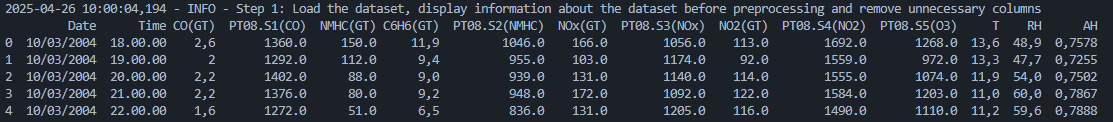
\includegraphics[width=0.9\textwidth]{images/raw_data_preview.png}
    \vspace{0.5cm}
    \caption{Hiển thị dữ liệu gốc trước khi tiền xử lý}
    \label{fig:raw_data_preview}
\end{figure}

\begin{figure}[htbp]
    \centering
    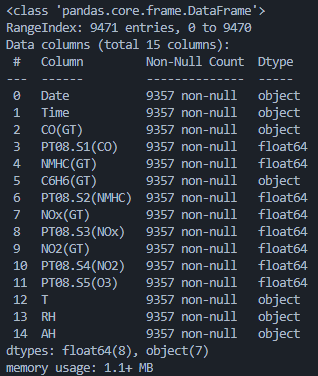
\includegraphics[width=0.45\textwidth]{images/raw_data_statistics.png}
    \vspace{0.5cm}
    \caption{Thống kê mô tả dữ liệu gốc}
    \label{fig:raw_data_statistics}
\end{figure}

\subsection{Ý nghĩa của các đặc trưng}

\begin{description}
    \item[CO(GT)]: Nồng độ Carbon Monoxide trong không khí, được tính toán là trung bình theo giờ (hourly averaged). Dữ liệu này được thu thập từ một máy phân tích tham chiếu (reference analyzer), có độ chính xác cao. Nồng độ CO được đo bằng mg/m³ (miligram trên mét khối). Carbon monoxide (CO) là một khí độc, không mùi và không màu, có thể gây nguy hiểm nếu nồng độ trong không khí quá cao. Khi nồng độ CO vượt quá mức an toàn, nó có thể gây ra các triệu chứng như chóng mặt, đau đầu, và thậm chí là ngộ độc, nguy hiểm đến tính mạng nếu nồng độ quá cao.

    \item[PT08.S1(CO)]: Phản hồi cảm biến theo giờ (hourly averaged sensor response) của một cảm biến được thiết kế để đo nồng độ khí carbon monoxide (CO). Dữ liệu này là giá trị đo được từ một cảm biến cụ thể (có thể là cảm biến điện hóa hoặc cảm biến quang học) được sử dụng để đo nồng độ CO. Cảm biến này không đo trực tiếp nồng độ CO bằng đơn vị mg/m³ hoặc ppm, mà thay vào đó là đo phản hồi của cảm biến (có thể là tín hiệu điện hay tín hiệu quang học).

    \item[NMHC(GT)]: Nồng độ trung bình theo giờ của các hợp chất hữu cơ không bão hòa (Non-Methane Hydrocarbons - NMHC) trong không khí. Dữ liệu này được thu thập từ một máy phân tích tham chiếu (reference analyzer), và giá trị trong cột này là nồng độ của các hợp chất này, đo bằng microgram mỗi mét khối (µg/m³). NMHC là một nhóm các hợp chất hữu cơ dễ bay hơi (VOCs) không chứa metan. Những hợp chất này thường xuất hiện trong khí thải từ các nguồn như giao thông, công nghiệp, hoặc từ các sản phẩm tiêu dùng như sơn và dung môi.

    \item[C6H6(GT)]: Nồng độ trung bình theo giờ của Benzen (C6H6) trong không khí, đo bằng microgram mỗi mét khối (µg/m³). Benzen là một hợp chất rất nguy hiểm nếu tiếp xúc lâu dài hoặc với nồng độ cao. Nó có thể gây ra các vấn đề nghiêm trọng về sức khỏe, bao gồm các bệnh về máu, ung thư và các vấn đề liên quan đến hệ thần kinh.

    \item[PT08.S2(NMHC)]: Phản hồi cảm biến theo giờ của một cảm biến được thiết kế để đo nồng độ các hợp chất hữu cơ không bão hòa (Non-Methane Hydrocarbons - NMHC) trong không khí. Dữ liệu này không đo nồng độ NMHC trực tiếp bằng các đơn vị như µg/m³ hay ppm, mà là giá trị phản hồi của cảm biến.

    \item[NOx(GT)]: Nồng độ trung bình theo giờ của Nitrogen Oxides (NOx) trong không khí, được đo bằng một máy phân tích tham chiếu. Đơn vị đo trong cột này là ppb (parts per billion). NOx là một nhóm các hợp chất bao gồm Nitrogen Dioxide (NO2) và Nitric Oxide (NO), có thể gây ảnh hưởng đến sức khỏe con người và môi trường.

    \item[PT08.S3(NOx)]: Phản hồi cảm biến theo giờ của một cảm biến được thiết kế để đo nồng độ Nitrogen Oxides (NOx) trong không khí. Dữ liệu này là phản hồi của cảm biến, tính trung bình trong suốt một giờ.

    \item[NO2(GT)]: Nồng độ trung bình theo giờ của Nitrogen Dioxide (NO2) trong không khí, được đo bằng một máy phân tích tham chiếu. Đơn vị đo của cột này là microgram per cubic meter (µg/m³). NO2 là một chất ô nhiễm quan trọng trong không khí, có thể gây ra các vấn đề sức khỏe nghiêm trọng.

    \item[PT08.S4(NO2)]: Phản hồi cảm biến theo giờ của một cảm biến được thiết kế để đo nồng độ Nitrogen Dioxide (NO2) trong không khí. Dữ liệu này là phản hồi cảm biến, tính trung bình trong suốt một giờ.

    \item[PT08.S5(O3)]: Phản hồi cảm biến theo giờ của một cảm biến được thiết kế để đo nồng độ Ozone (O3) trong không khí. Dữ liệu này là phản hồi của cảm biến, được tính trung bình trong suốt một giờ.

    \item[T]: Nhiệt độ (Temperature) trong không khí, được đo bằng đơn vị độ Celsius (°C). Nhiệt độ đóng vai trò quan trọng trong việc xác định điều kiện môi trường và ảnh hưởng đến sự phân tán và pha loãng các chất ô nhiễm.

    \item[RH]: Độ ẩm tương đối (Relative Humidity), được đo bằng đơn vị % (phần trăm). Đây là tỷ lệ giữa lượng hơi nước hiện có trong không khí và lượng hơi nước tối đa mà không khí có thể chứa tại một nhiệt độ nhất định. Độ ẩm tương đối ảnh hưởng lớn đến chất lượng không khí và các phản ứng hóa học trong khí quyển.

    \item[AH]: Độ ẩm tuyệt đối (Absolute Humidity), được đo bằng đơn vị g/m³ (gram trên mét khối). Đây là lượng hơi nước có trong không khí, không phụ thuộc vào nhiệt độ. Độ ẩm tuyệt đối là một chỉ số quan trọng để hiểu rõ hơn về sự thay đổi của lượng hơi nước trong không khí và ảnh hưởng của nó đến chất lượng không khí.

    \item[Date\_Time]: Thời gian đo đạc
    \item[Year, Month, Day, Hour]: Các đặc trưng thời gian
\end{description}

\subsection{Quá trình tiền xử lý dữ liệu}

\subsubsection{Bước 1: Xử lý các cột không cần thiết}
\hspace{0.5cm}Đầu tiên, nhóm loại bỏ các cột không cần thiết như "Unnamed: 15" và "Unnamed: 16" để làm sạch dữ liệu.

\subsubsection{Bước 2: Xử lý giá trị thiếu}
\hspace{0.5cm}Đối với các cột số học, giá trị thiếu được thay thế bằng giá trị trung bình của cột đó. Đối với các cột dạng chuỗi, giá trị thiếu được thay thế bằng giá trị xuất hiện thường xuyên nhất.

\subsubsection{Bước 3: Chuyển đổi kiểu dữ liệu}
\hspace{0.5cm}Các cột dữ liệu được chuyển đổi sang kiểu dữ liệu phù hợp:
\begin{itemize}
    \item Cột "Date" được chuyển đổi từ định dạng DD/MM/YYYY sang datetime
    \item Cột "Time" được chuyển đổi từ định dạng HH.MM.SS sang time
    \item Các cột số học được chuẩn hóa bằng cách thay thế dấu phẩy bằng dấu chấm
    \item Cột CO(GT) có giá trị -200 được thay thế bằng giá trị trung bình
\end{itemize}

\subsubsection{Bước 4: Xử lý ngoại lệ (outliers)}
\hspace{0.5cm}Nhóm sử dụng phương pháp Z-score để xác định và xử lý các giá trị ngoại lệ:
\begin{itemize}
    \item Tính toán Z-score cho mỗi cột số học
    \item Xác định ngưỡng là 3 độ lệch chuẩn
    \item Thay thế các giá trị ngoại lệ bằng giá trị trung bình của cột
    \item Đặc biệt xử lý cột NMHC(GT) để đảm bảo không có giá trị âm
\end{itemize}

\begin{figure}[htbp]
    \centering
    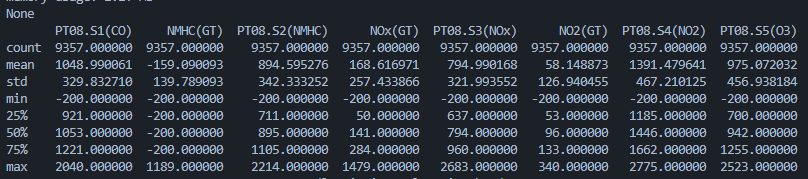
\includegraphics[width=0.9\textwidth]{images/data_distribution_comparison.png}
    \vspace{0.5cm}
    \caption{So sánh phân phối dữ liệu trước và sau khi xử lý ngoại lệ}
    \label{fig:data_distribution}
\end{figure}

\subsubsection{Bước 5: Tạo đặc trưng mới}
\hspace{0.5cm}Nhóm tạo các đặc trưng mới từ dữ liệu hiện có:
\begin{itemize}
    \item Kết hợp cột "Date" và "Time" thành cột "Date\_Time"
    \item Trích xuất thông tin năm, tháng, ngày và giờ từ cột "Date\_Time"
    \item Tạo các đặc trưng tương tác như Temp\_Humidity, NOx\_NO2
    \item Thêm các đặc trưng thống kê như rolling mean và rolling std
\end{itemize}

\subsection{Kết quả tiền xử lý dữ liệu}

\subsubsection{Thông tin tổng quan về dữ liệu}
\hspace{0.5cm}Sau khi tiền xử lý, bộ dữ liệu có các đặc điểm sau:
\begin{itemize}
    \item Số lượng mẫu: 9,471
    \item Số lượng đặc trưng: 18
    \item Các kiểu dữ liệu:
    \begin{itemize}
        \item float64: 13 cột
        \item datetime64[ns]: 1 cột
        \item int32: 4 cột
    \end{itemize}
\end{itemize}

\begin{figure}[htbp]
    \centering
    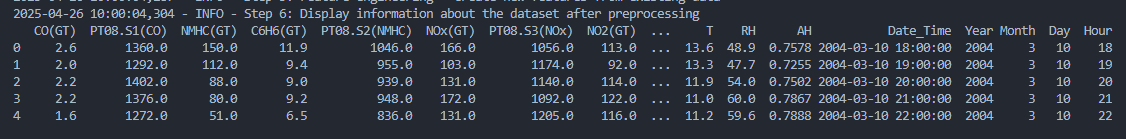
\includegraphics[width=0.9\textwidth]{images/processed_data_preview.png}
    \vspace{0.5cm}
    \caption{Hiển thị dữ liệu sau khi tiền xử lý}
    \label{fig:processed_data_preview}
\end{figure}

\subsubsection{Thống kê mô tả}
\hspace{0.5cm}Các thống kê chính của dữ liệu sau tiền xử lý:
\begin{itemize}
    \item CO(GT): Giá trị trung bình 0.77, dao động từ -5.12 đến 11.90
    \item PT08.S1(CO): Giá trị trung bình 1097.15, dao động từ 647 đến 2008
    \item NMHC(GT): Giá trị trung bình 213.58, dao động từ 29 đến 405
    \item C6H6(GT): Giá trị trung bình 10.06, dao động từ 0.10 đến 63.70
\end{itemize}

\begin{figure}[htbp]
    \centering
    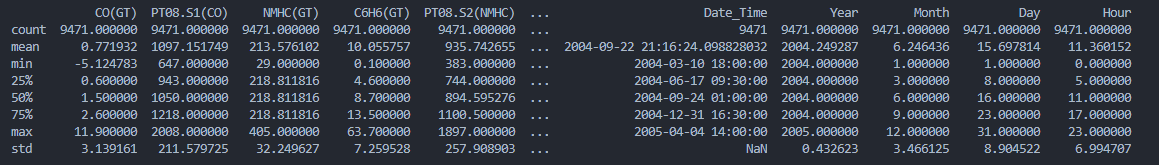
\includegraphics[width=0.45\textwidth]{images/processed_data_statistics.png}
    \vspace{0.5cm}
    \caption{Thống kê mô tả dữ liệu sau tiền xử lý}
    \label{fig:processed_data_statistics}
\end{figure}

\subsection{Kết luận}
\hspace{0.5cm}Quá trình tiền xử lý dữ liệu đã giúp chuẩn bị bộ dữ liệu chất lượng không khí cho việc xây dựng mô hình học máy. Các bước xử lý đã giải quyết các vấn đề về giá trị thiếu, ngoại lệ và tạo thêm các đặc trưng có ý nghĩa. Kết quả cho thấy dữ liệu đã được chuẩn hóa và sẵn sàng cho việc huấn luyện mô hình.
\newpage
%%%%%%%%%%%%%%%%%OUTRO%%%%%%%%%%%%%%%%%%%
\input{Outro/TaiLieuThamKhao}
\newpage
\input{Outro/PhuLuc}
\end{document}
